\documentclass[aspectratio=169]{beamer}

% Packages
\usepackage{amsthm}        % For theorems
\usepackage{amsmath}       % For math
\usepackage{luatexja}      % For Japanese
\usepackage{booktabs}      % For formal tables
\usepackage{mathtools}
\usepackage{amssymb}       % For checkmark
\usepackage{ulem}          % For strikeout
\usepackage[dvipsnames]{xcolor} % For colors (i.e. ForestGreen)
\usepackage[noend]{algpseudocode}
\usepackage[backend=biber,
            style=authoryear,
            sorting=none
            ]{biblatex}    % For bibliography
\usepackage{tikz}          % For figures
\usepackage{multirow}      % For multiorow in tables
\usepackage{xspace}            % For proper spacing after macros
\usepackage{thmtools}
\usepackage{thm-restate}
\usetikzlibrary{arrows.meta,
                chains,
                positioning}

\addbibresource{references.bib}

% Settings for bibliography
\renewcommand*{\mkbibparens}[1]{\mkbibbrackets{#1}}
\renewcommand*{\nameyeardelim}{\addcomma\space}

% Custom commands
\DeclareMathOperator{\interior}{int}
\DeclareMathOperator{\sgn}{sgn}

% Macro
\newcommand{\cost}{\text{cost}}
\newcommand{\costassign}[1]{\text{cost}_{assign}{#1}}
\newcommand{\costopen}[1]{\text{cost}_{open}{#1}}
\newcommand{\opt}{(S^*, \sigma^*)}
\newcommand*{\localopt}{(S, \sigma)}
\newcommand{\ALG}{\text{\upshape ALG}\xspace}
\newcommand{\OPT}{\text{\upshape OPT}\xspace}

\newcommand{\FacilitySet}{\mathcal{F}}
\newcommand{\DemandSet}{\mathcal{D}}
\newcommand{\isafe}{\info{i_{\text{safe}}}}
\newcommand{\iunsafe}{\alert{i_{\text{unsafe}}}}

% Beamer settings
\usepackage{caption}
\captionsetup[figure]{labelformat=empty}

% \setbeamertemplate{theorems}[numbered]
\addtobeamertemplate{theorem begin}{\normalfont}{}
\newtheorem*{theorem*}{Theorem (restated)}
\newtheorem*{lemma*}{Lemma (restated)}
\newtheorem*{sproof}{Sketch of the proof.}
\newtheorem{remark}[theorem]{Remark}
\newtheorem{observation}[theorem]{Observation}

% \setbeameroption{hide notes}
% \setbeameroption{show only notes}
\setbeameroption{show notes on second screen=right}

\newcommand{\info}[1]{\textcolor{ForestGreen}{#1}}
\newcommand{\out}[1]{\textcolor{lightgray}{#1}}

% Theme
\usetheme[
    block=fill,
    % progressbar=foot,
    % numbering=fraction,
]{metropolis}
\usecolortheme{default}

% Fonts
\setbeamerfont{title}{size=\large,series=\bfseries}
\setbeamerfont{theorem}{shape=\upshape}
\usefonttheme{professionalfonts}
\usefonttheme{structurebold}
\setbeamerfont{title}{size=\LARGE}
\setbeamerfont{date}{size=\small}
\setbeamerfont{frametitle}{size=\large,series=\bfseries}
\setmainfont{Latin Modern Roman}
\usepackage{luatexja-fontspec}
\usepackage[T1]{fontenc}
\usepackage{mlmodern}
\usepackage{luatexja-otf}
\renewcommand{\kanjifamilydefault}{\gtdefault} % 既定欧文フォントがサンセリフなので，既定和文フォントもゴシック体に設定する
\renewcommand{\familydefault}{\sfdefault}

% Metadata
\title{7.8 施設配置問題に対する局所探索アルゴリズム}
\subtitle{近似アルゴリズム ―離散最適化問題への効果的アプローチ―}
\author{岡山 大輝}
\institute{兵庫県立大学大学院 情報科学研究科\textit{(ad25r010@guh.u-hyogo.ac.jp)}}
\date{January 5 \& January 12, 2026}

\begin{document}

\begin{frame}
  \titlepage
\end{frame}

\section{施設配置問題と局所探索アルゴリズム}

\begin{frame}{施設配置問題（Uncapacitated Metric Facility Location）}
  本スライドでは，\alert{容量制限のないメトリック施設配置問題}を考える。

  \begin{itemize}
    \item \(\FacilitySet\)：施設集合，\(\DemandSet\)：需要（顧客）集合
    \item 各施設 \(i \in \FacilitySet\) には開設コスト \(f_i \ge 0\) が与えられている
    \item \(\FacilitySet \cup \DemandSet\) 上に距離関数
          \[
            c \colon (\FacilitySet \cup \DemandSet) \times (\FacilitySet \cup \DemandSet) \to \mathbb{R}_{\ge 0}
          \]
          が定義されている
    \item 距離 \(c(\cdot,\cdot)\) はメトリック
          （非負性・対称性・三角不等式）を満たす
  \end{itemize}
  \vskip 1em

  \usebeamercolor{block body}
  \begin{beamercolorbox}[
      wd=\linewidth,
      sep=1ex,
      leftskip=1ex,
      rightskip=1ex,
      colsep*=0pt,
    ]{block body}
    \textbf{目的：}\;
    開設コストと割当コストの総和を最小化する
  \end{beamercolorbox}

  \vskip -1em

  \[
    \min_{S \subseteq \FacilitySet,\;\sigma \colon \DemandSet \to S}
    \left(
    \sum_{i \in S} f_i
    \;+\;
    \sum_{j \in \DemandSet} c_{\sigma(j)j}
    \right)
  \]

  \note{
    \begin{itemize}
      \item 解は「開設する施設集合 \(S\)」と「割当 \(\sigma\)」の組で表される
      \item 局所探索では，この \((S,\sigma)\) を少しずつ変更して改善を試みる
    \end{itemize}
  }
\end{frame}

\begin{frame}{施設配置問題に対する局所探索アルゴリズム}
  適当な非空集合から開始し、追加／削除／交換移動をコストが改善する限り繰り返す。

  \begin{figure}
    \centering
    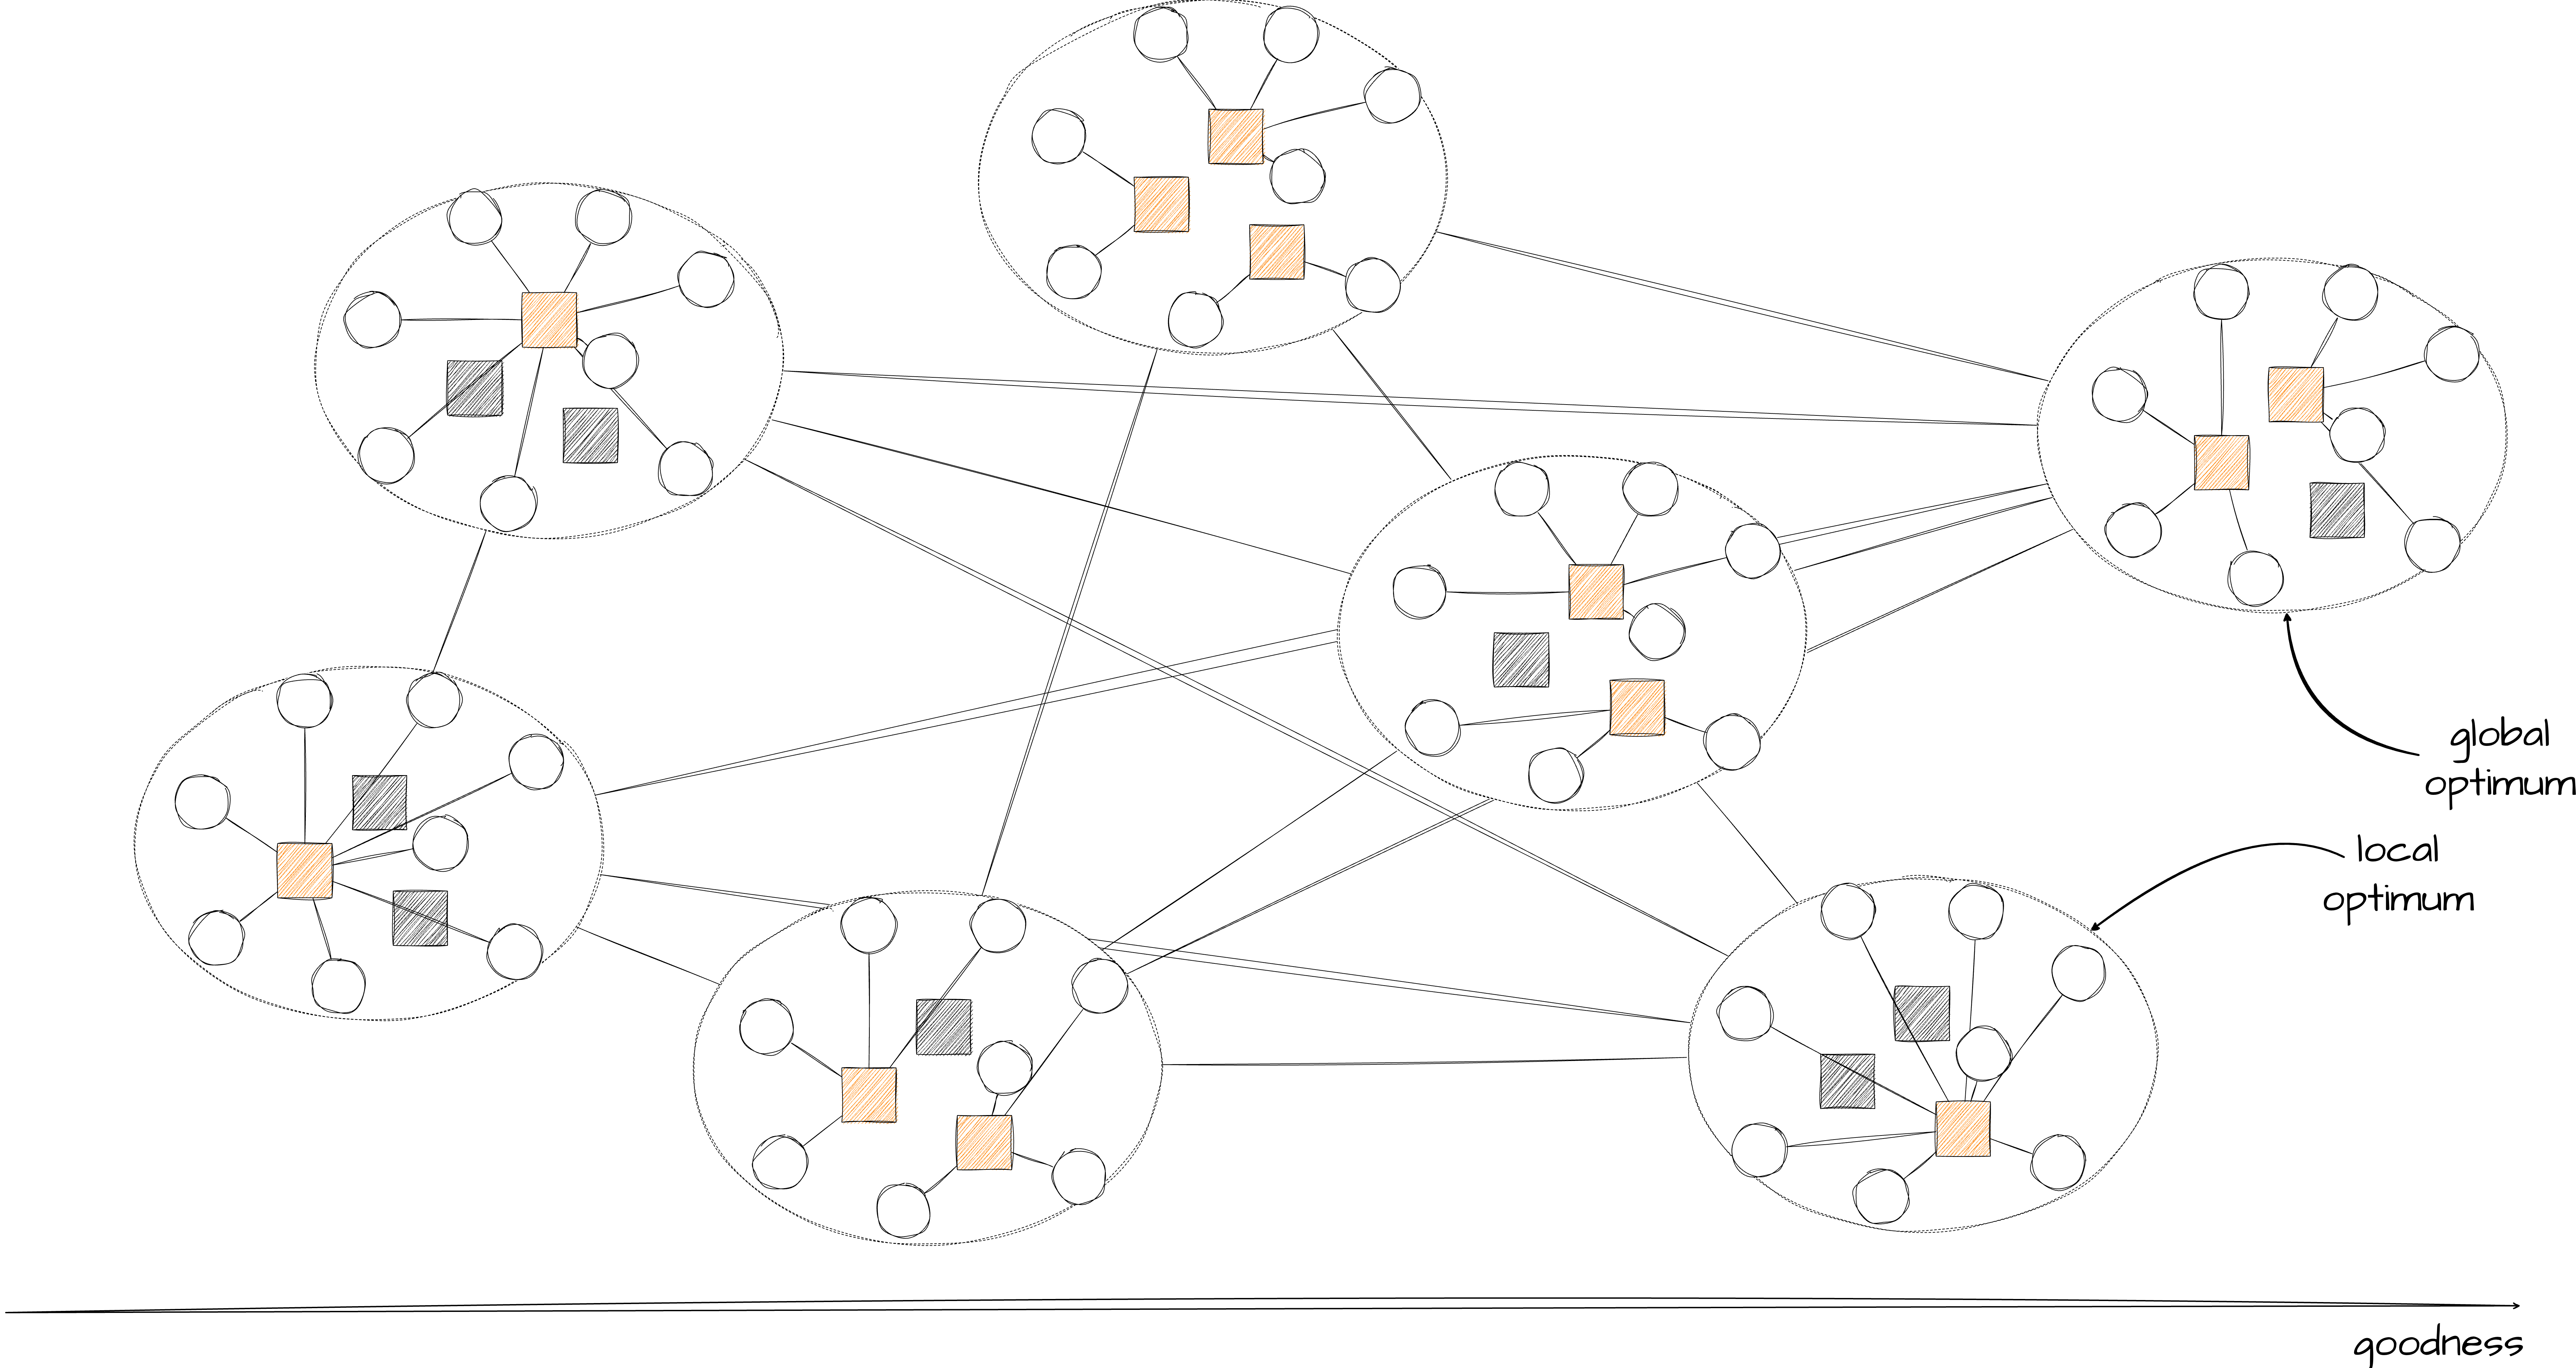
\includegraphics[width=0.9\textwidth]{figures/neighborhood.drawio.png}
  \end{figure}

  \note{
    \begin{itemize}
      \item
    \end{itemize}
  }
\end{frame}

\section{局所最適解の解析}

\begin{frame}{施設配置問題に対する局所最適解の性質}
  \begin{lemma}
    局所最適解 \(\localopt\) に対して、
    \(C \le F^* + C^* = \OPT\)
    が成立する。
  \end{lemma}

  \begin{lemma}[後で示す]
    局所最適解 \(\localopt\) に対して、
    \(F \le F^* + 2C^*\)
    が成立する。
  \end{lemma}

  \begin{theorem}[\cite{arya2004local}]
    施設配置問題の局所最適解 \(\localopt\) の総コストは、高々 \(3\OPT\) である。
  \end{theorem}

  \textbf{Proof. } 局所最適解の総コストは \(C + F\) であり、上の 2 つの補題より、
  \[C + F \le (F^* + C^*) + (F^* + 2C^*) = 2F^* + 3C^* < 3F^* + 3C^* = 3\OPT.\]

  \note{
    \begin{itemize}
      \item いろいろ示唆に富んだ補題
      \item 任意の最適解に対してこの補題が成り立つという点
      \item \(F^* + C^*\) が一致すればよいので、極端な話、\(F^*\) が非常に大きく \(C^*\) が非常に小さい場合ような最適解に対しても成り立つ
    \end{itemize}
  }
\end{frame}

\begin{frame}{施設配置問題に対する局所最適解のタイトな例}

  局所最適解の総コストが最適値の少なくとも \(3 - o(1)\) 倍になる例~(\cite{arya2004local})．
  \begin{figure}
    \centering
    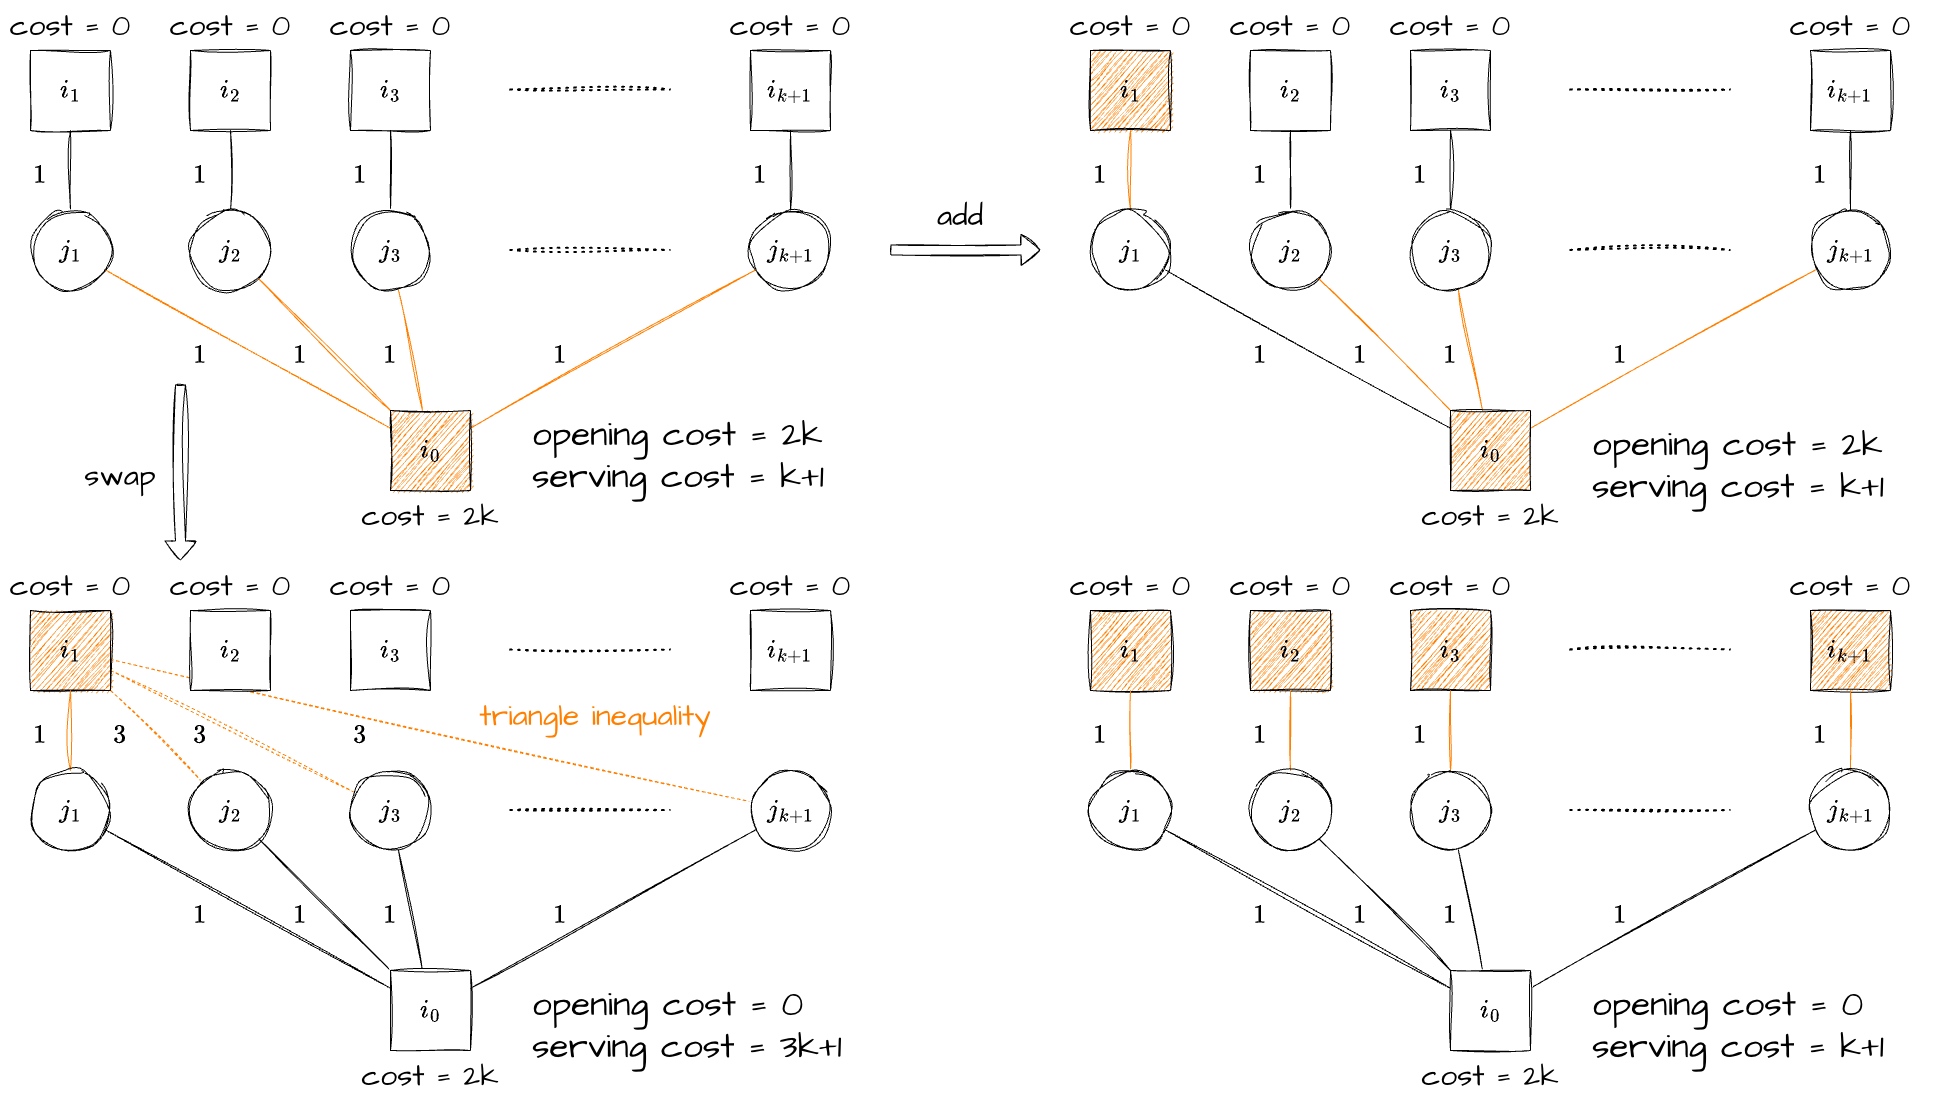
\includegraphics[width=0.85\textwidth]{figures/lower-bound.drawio.png}
  \end{figure}

  \note{
    \begin{itemize}
      \item まずインスタンスの説明（開設コスト \(0\) の施設が \(k+1\) 個，開設コスト \(2k\) の施設が \(1\) 個，顧客が \(k+1\) 人、すべての距離が \(1\) であること）
      \item 施設 \(i_0\) を開設し、各顧客をそれぞれの施設に割り当てる解のコストが \(2k + (k+1) = 3k + 1\) であること
      \item 追加操作、交換操作によって解の値が改善されないので、これは局所最適解であること
      \item 最適解は、施設 \(i_0\) 以外の施設をすべて開設し、各顧客をそれぞれの施設に割り当てる解であり、そのコストは \(k + 1\) であること
    \end{itemize}
  }
\end{frame}

\subsection{割り当てコストの上界}

\subsection{開設コストの上界}

\begin{frame}{開設コストの上界}
  \begin{lemma}
    局所最適解 \(\localopt\) に対して、
    \(F \le F^* + 2C^*\)
    が成立する。
  \end{lemma}

  \textbf{Sketch of the proof. }
  局所最適解に対する追加／削除／交換移動によって、コストが改善しないことから導かれる不等式を組み合わせて示す。
  \begin{itemize}
    \leftskip 2em
    \item[（削除） ] \(0 \le -f_i + \sum_{j \in D \colon \sigma(j) = i} 2c_{\sigma^*(j)j}\)
    \item[（追加） ] \(0 \le f_{i^*} + \sum_{j \in D \colon \sigma(j) = i \text{ and } \sigma^*(j) = i^*} (c_{\sigma^*(j)j} - c_{\sigma(j)j})\)
    \item[（交換） ] \(0 \le f_{i^{'}} - f_i + \sum_{j \in D \colon \sigma(j) = i \text{ and } \sigma^*(j) \in R_i} (c_{i'j} - c_{\sigma(j)j}) + \sum_{j \in D \colon \sigma(j) = i \text{ and } \sigma^*(j) \notin R_i} 2c_{\sigma^*(j)j}\)
  \end{itemize}
\end{frame}

\begin{frame}{準備：再割当てにおけるコストの増加分の上界}
  \begin{lemma}
    施設 \(\sigma(j) = i\) と \(i' = \phi(\sigma^*(j))\) が異なるような任意の利用者 \(j\) を考える。\\
    このとき、利用者 \(j\) を施設 \(i\) から施設 \(i'\) に再割当てしたときのコストの増加分 (\(c_{i'j} - c_{ij}\)) は、
    高々 \(2c_{\sigma^*(j)j}\) である。
  \end{lemma}

  \begin{columns}
    \begin{column}{0.45\textwidth}
      \begin{figure}
        \centering
        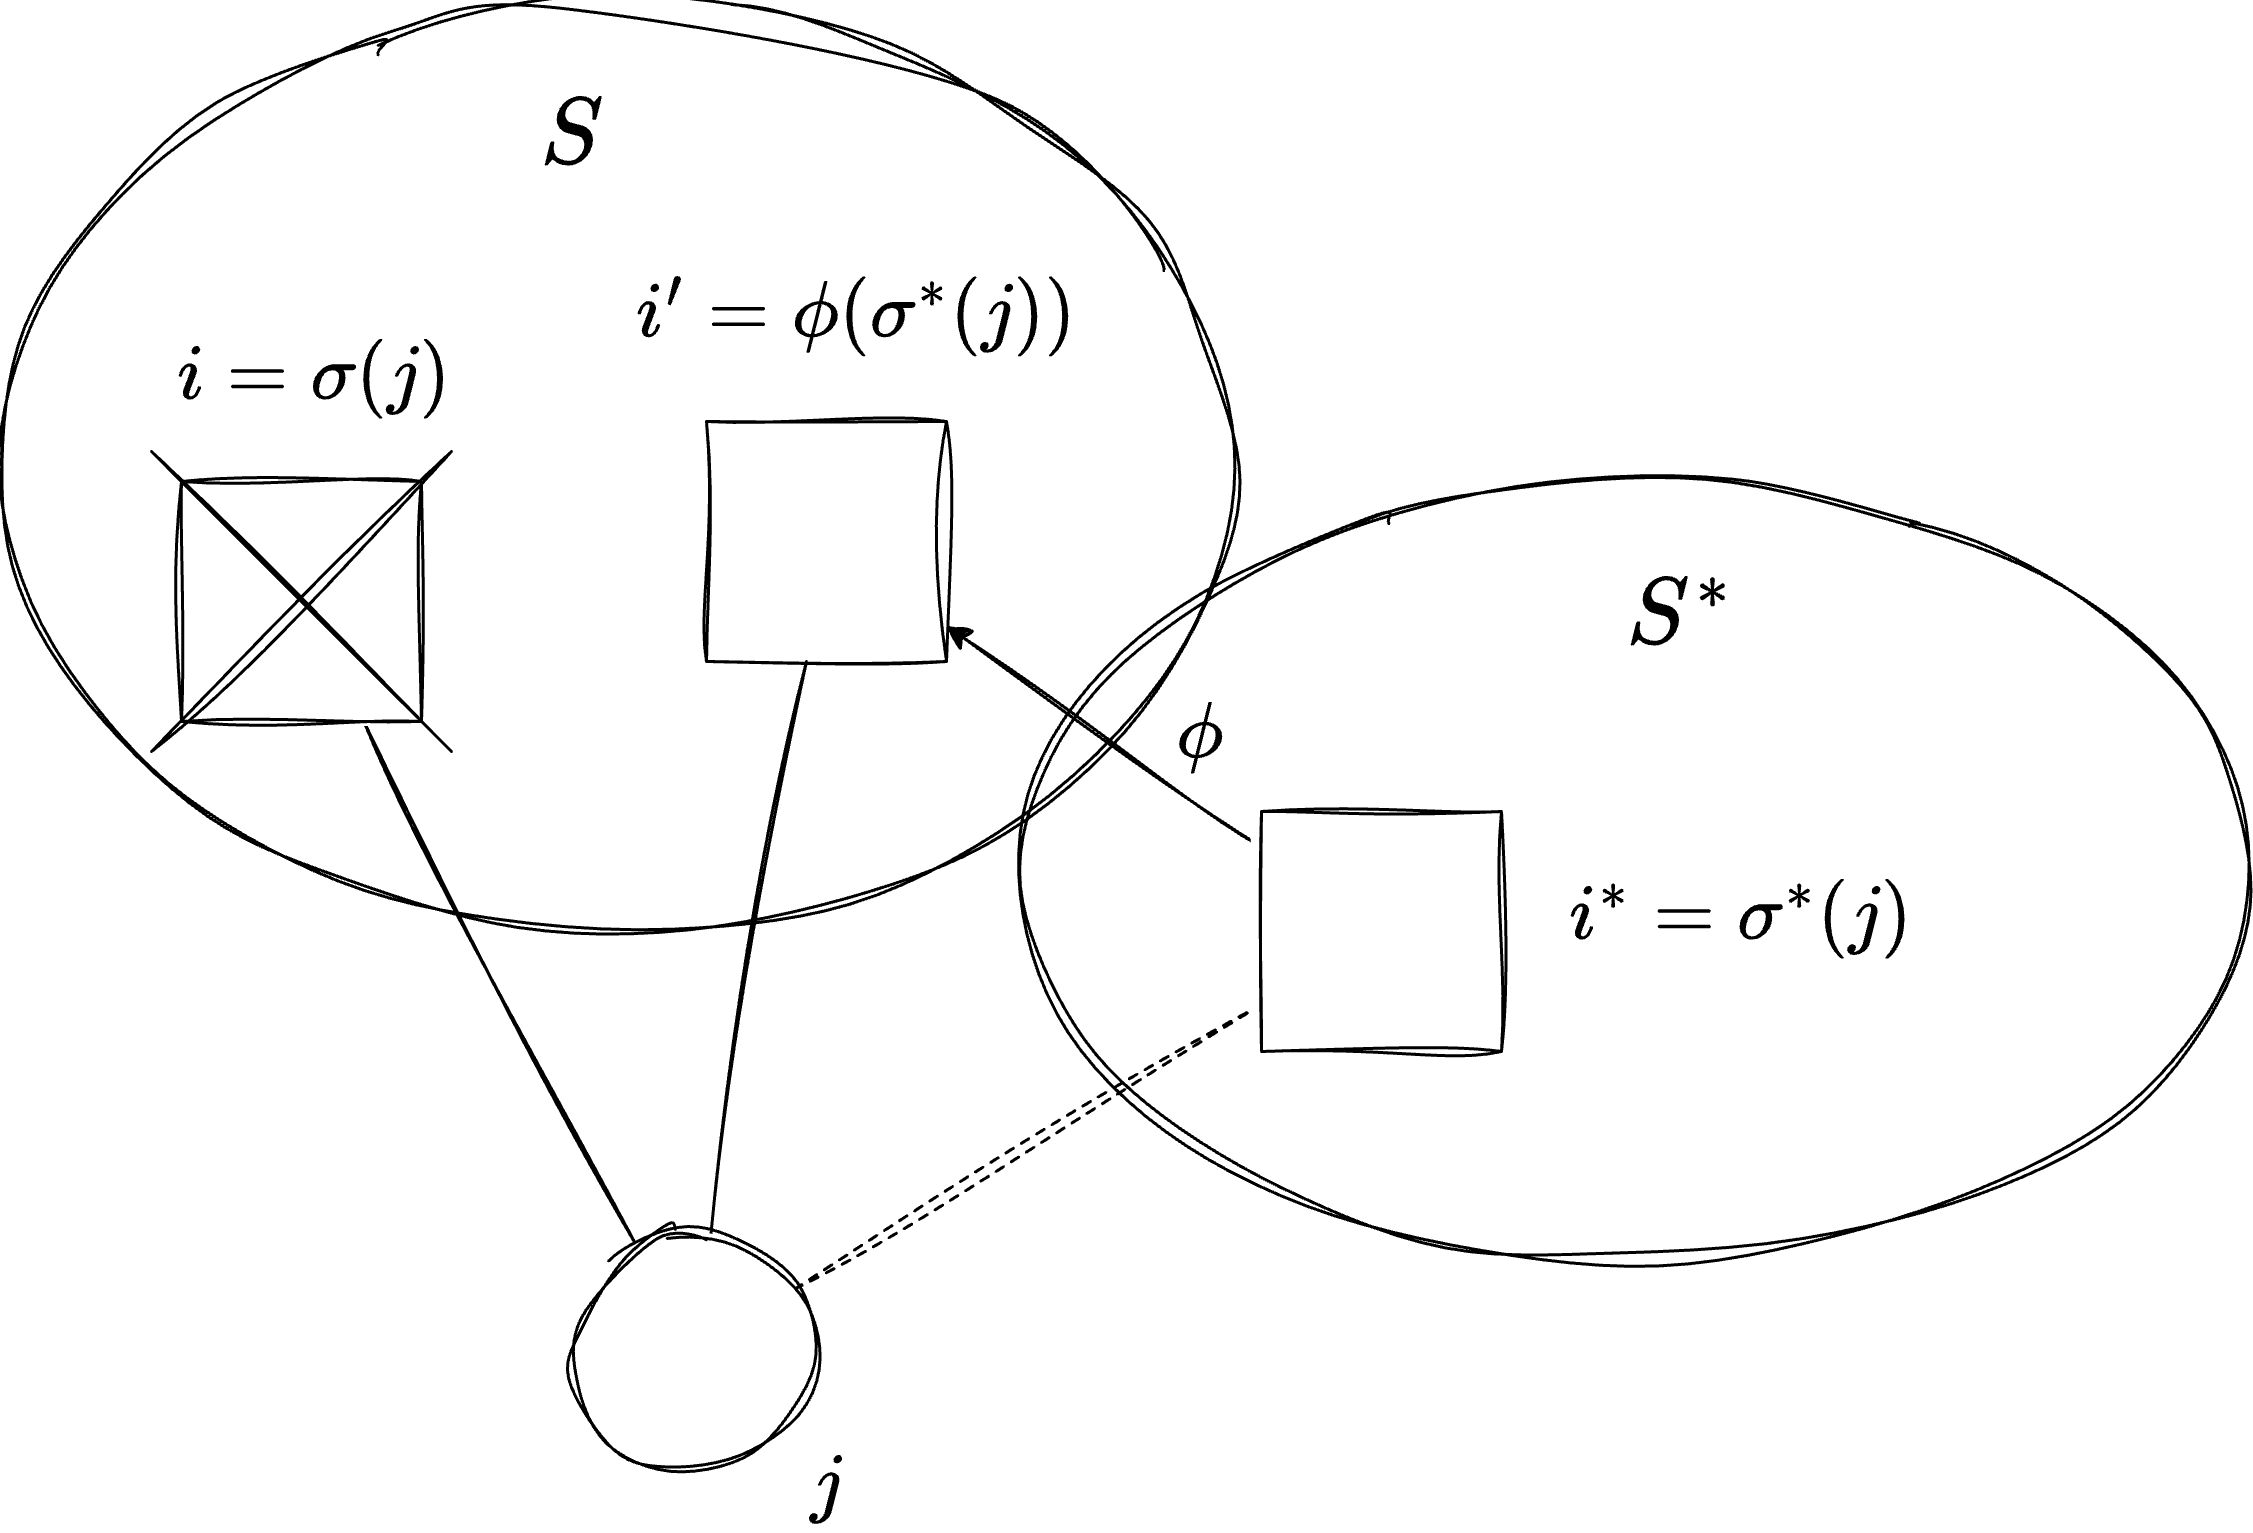
\includegraphics[width=\textwidth]{figures/reassignment.drawio.png}
      \end{figure}
    \end{column}
    \begin{column}{0.45\textwidth}
      \begin{figure}
        \centering
        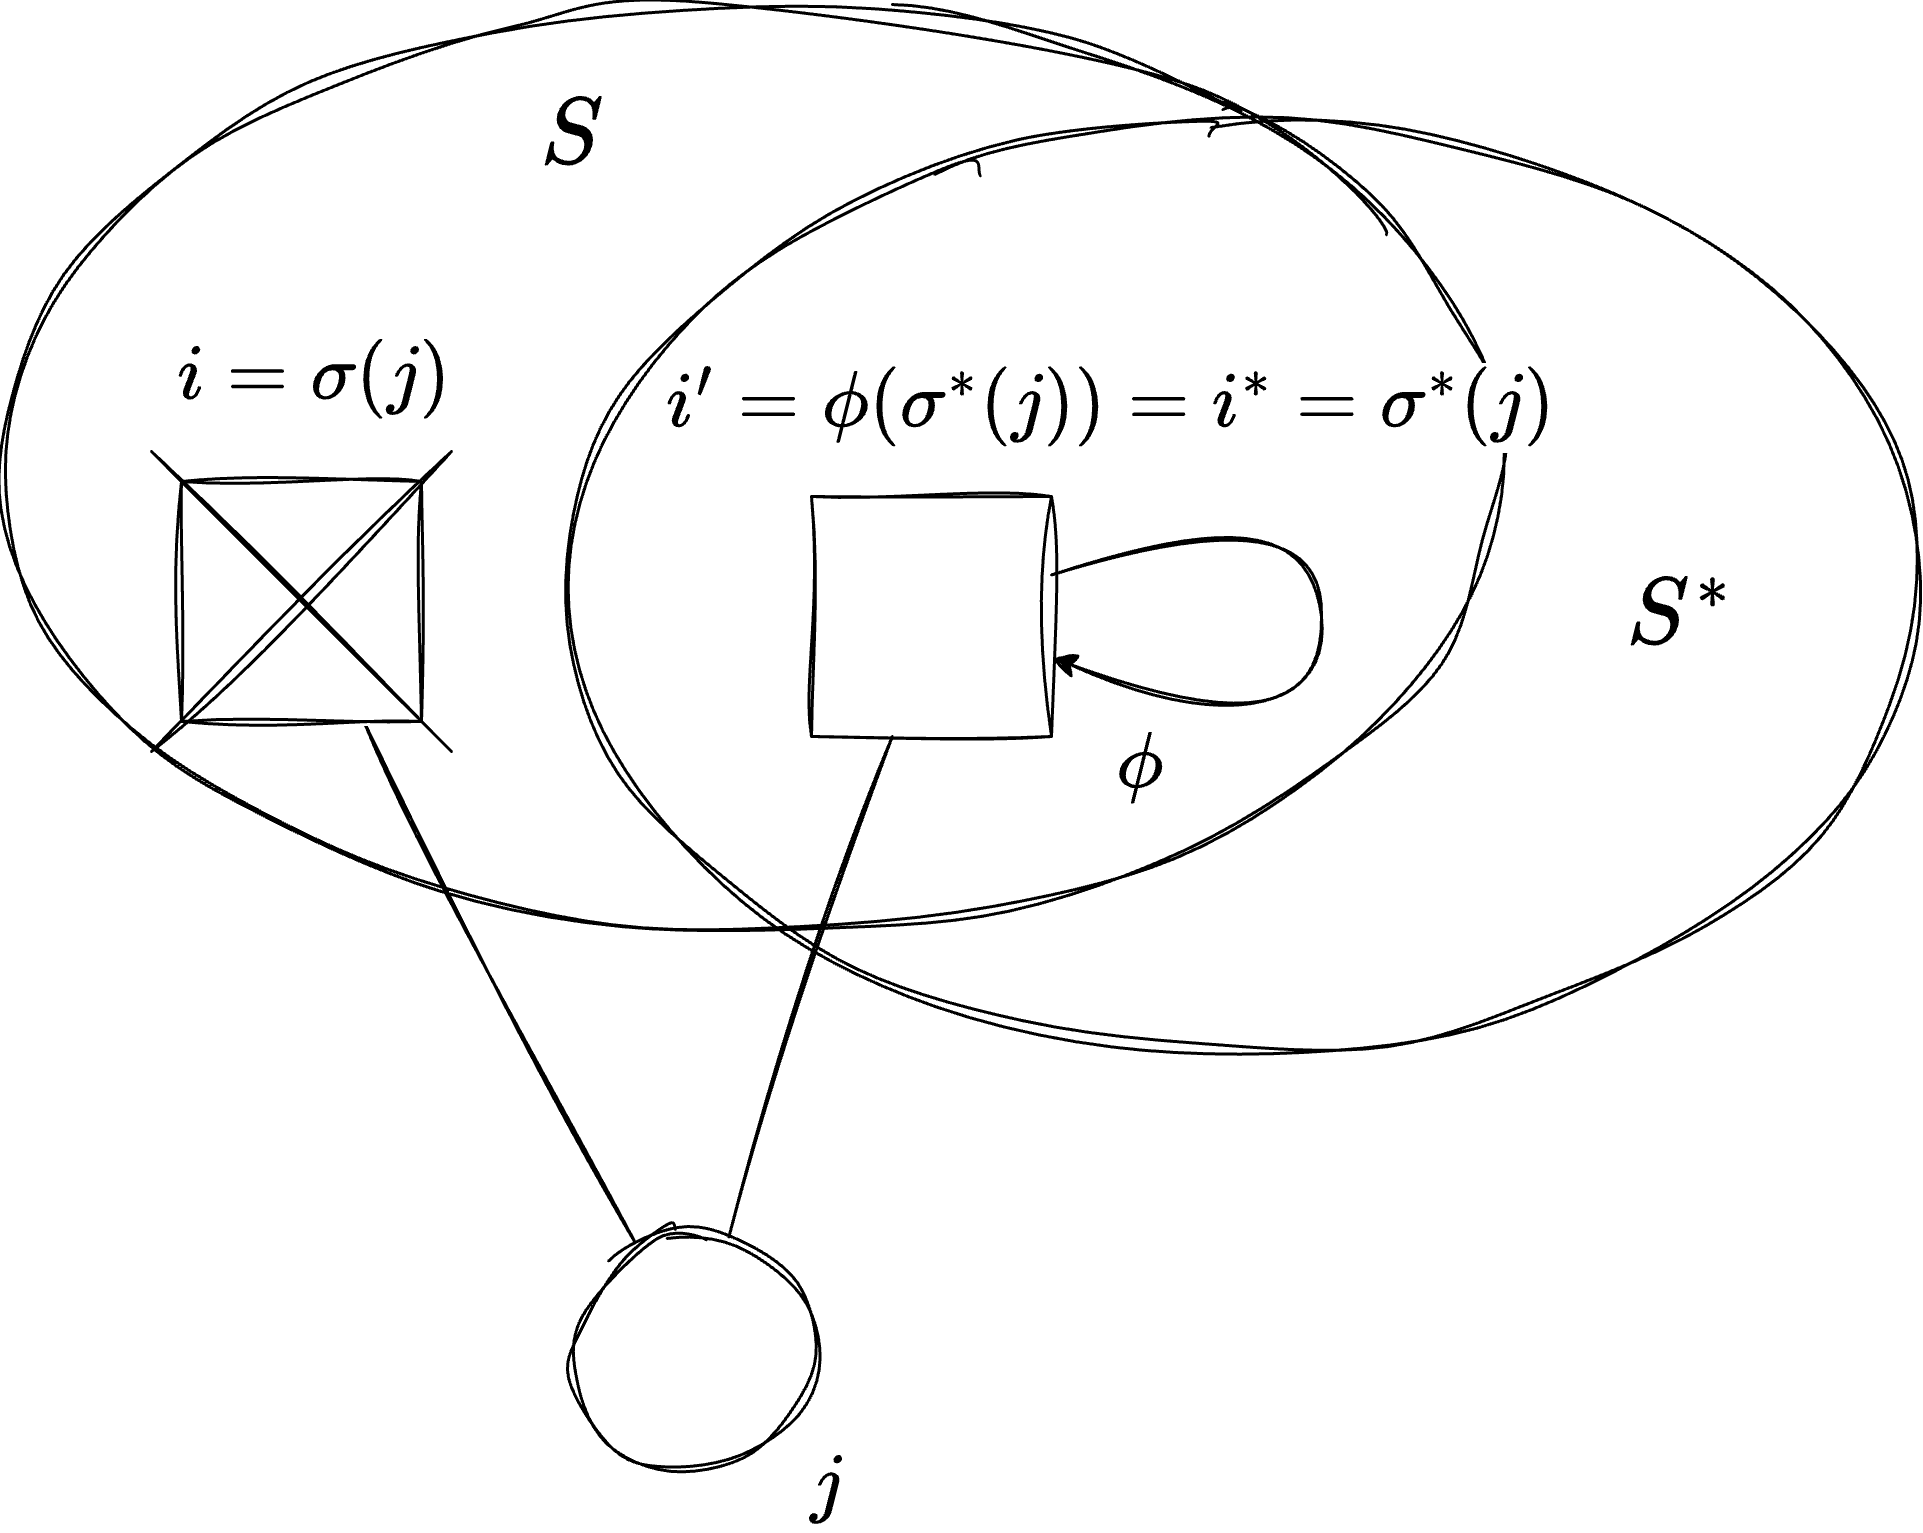
\includegraphics[width=\textwidth]{figures/reassignment-case2.drawio.png}
      \end{figure}
    \end{column}
  \end{columns}


  \note{
    \begin{itemize}
      \item これから削除移動や交換移動を考えるが、今割り当てられている施設が閉じてしまった場合に、他の開設している施設に割り当て直す必要がある
      \item その施設の決め方としてあり得るものは、最適解において割り当てられていた施設から最も近い施設に割り当て直す方法である（もちろんそのような施設が存在すれば）
      \item 直感的にはそこまで悪くなさそうで、実際に三角不等式によって上界を与えることができるというのがこの補題
    \end{itemize}
    ---
    \begin{itemize}
      \item なお \(i \in S^*\) のときでも成り立つよね？？
    \end{itemize}
  }
\end{frame}

\begin{frame}{準備：安全な施設と安全でない施設}
  \begin{columns}
    \begin{column}{0.45\textwidth}
      \begin{figure}
        \centering
        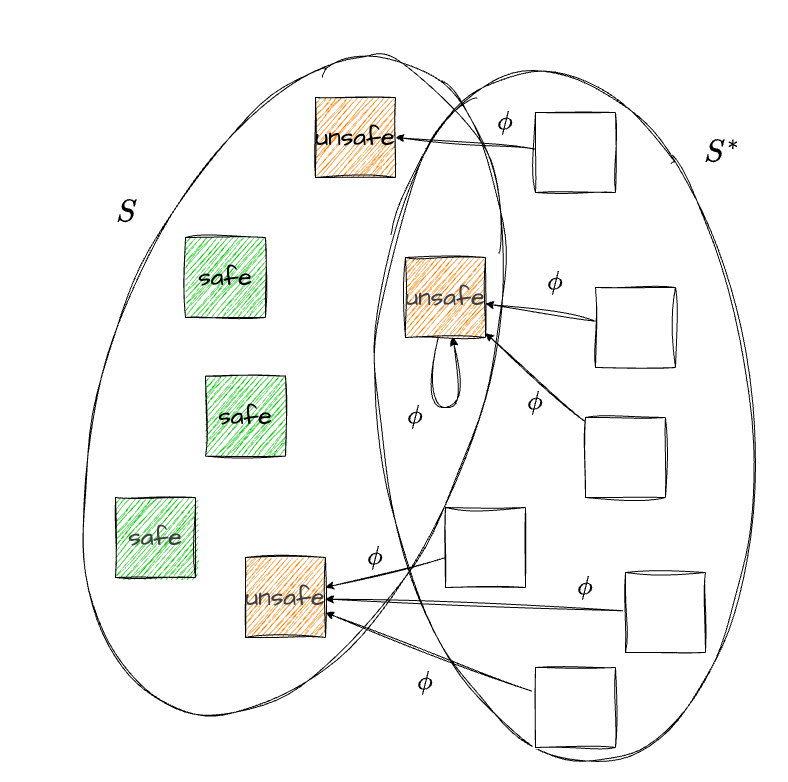
\includegraphics[width=\textwidth]{figures/safe-facility.drawio.png}
      \end{figure}
    \end{column}
    \begin{column}{0.45\textwidth}
      \begin{definition}[安全な施設]
        施設 \(i \in S\) が\info{安全}であるとは、
        最適解の全ての施設 \(i^* \in S^*\) について、
        \[
          \phi(i^*) \neq i
        \]
        が成立することである。
      \end{definition}
      逆に、ある施設 \(i^* \in S^*\) について、
      \[
        \phi(i^*) = i
      \]
      が成立する場合、施設 \(i\) を\alert{安全でない}とよぶ。
    \end{column}
  \end{columns}

  \note{
    \begin{itemize}
      \item 何に対して安全／安全でないと言っているのかは次のスライドですぐに明らかになる
      \item ネタバレすると、安全な施設はすべて削除移動の対象となる
      \item 安全でない施設と、\(S^*\) の最も最寄りの施設が交換移動の対象となる
      \item 残りの \(S^*\) の施設は追加移動の対象とな
    \end{itemize}
  }
\end{frame}

% \begin{frame}{補足：安全でない施設 \(i \in S \bigcap S^*\) に対する集合 \(R_i\) と施設 \(i'\)}
%   \begin{columns}
%     \begin{column}{0.45\textwidth}
%       \begin{figure}
%         \centering
%         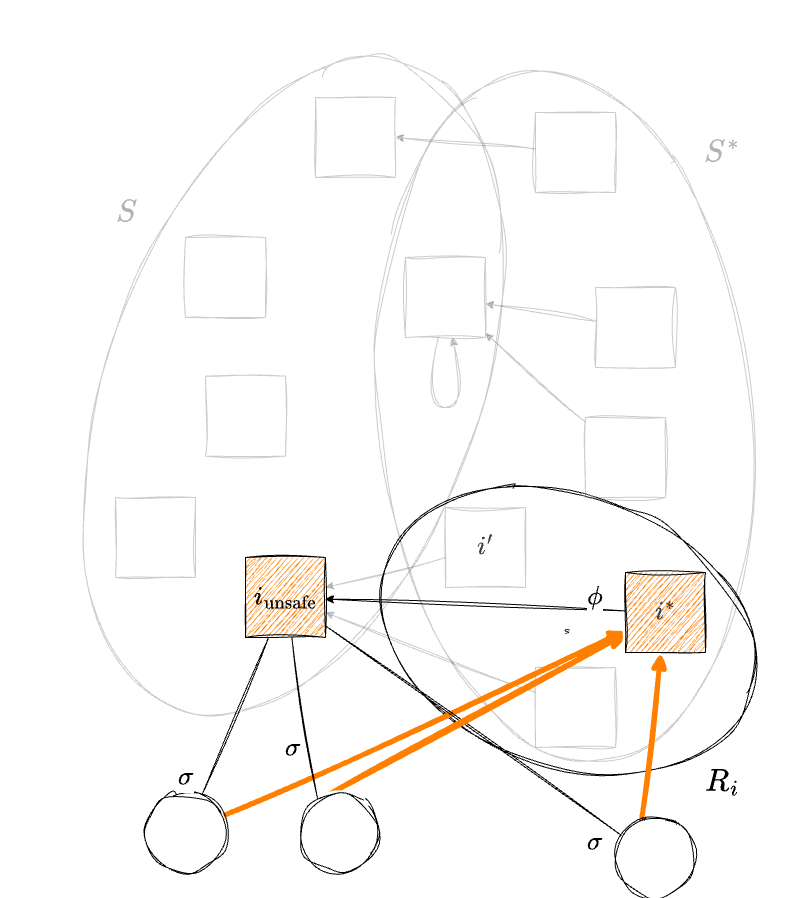
\includegraphics[width=\textwidth]{figures/unsafe-facility-add.drawio.png}
%       \end{figure}
%     \end{column}
%     \begin{column}{0.45\textwidth}
%       \begin{itemize}
%         \item \alert{安全でない施設} \(\alert{i} \in S \bigcap S^*\) を固定する
%         \item 最適解の施設 \(i^* \in S^*\) であって、\(\phi(i^*) = \alert{i}\) を満たすものを \(R_i (\subseteq S^*)\) とする
%               \begin{itemize}
%                 \item この場合、\(i \in R_i\)？
%               \end{itemize}
%         \item このとき、\(i' = i\) になるの？
%       \end{itemize}
%     \end{column}
%   \end{columns}
% \end{frame}

\begin{frame}{削除移動：\(S\) の安全な施設の削除と割り当ての変化}
  \begin{columns}
    \begin{column}{0.45\textwidth}
      \begin{figure}
        \centering
        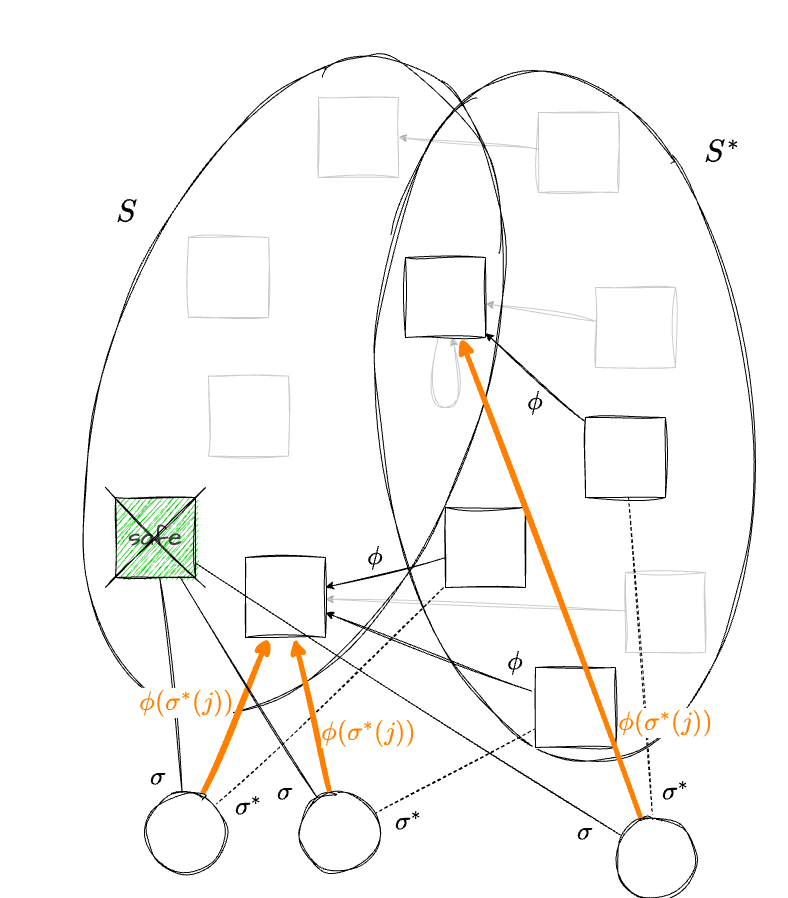
\includegraphics[width=\textwidth]{figures/safe-facility-delete.drawio.png}
      \end{figure}
    \end{column}

    \begin{column}{0.45\textwidth}
      \only<1>{
        \begin{itemize}
          \item \info{安全な施設} \(\info{i_{\text{safe}}} \in S\) を一つ選び削除
          \item \(\sigma(j) = \info{i_{\text{safe}}}\) を満たす利用者 \(j\) について割当てを変更：
                \begin{itemize}
                  \item 最適解において \(j\) が割り当てられていた施設 \( \sigma^*(j) \) に最も近い施設 \(\phi(\sigma^*(j))\) に再割当てする
                  \item 必ず \(\phi(\sigma^*(j)) \neq \info{i_{\text{safe}}}\)
                \end{itemize}
        \end{itemize}
      }
      \small{
        \only<2->{
          \vskip 0.5em
          次式が得られる：
          \begin{align*}
             & \underbrace{\sum_{i \in S} f_i + \sum_{j \in \DemandSet} c_{\sigma(j)j}}_{\text{局所最適解 } (S, \sigma) \text{ のコスト}}                                                                                                                                                                                                   \\
             & \left(\le \underbrace{S - \{\info{i_{\text{safe}}}\} \text{ の下で最適な割り当てをした解のコスト}}_{(S, \sigma) \text{ の近傍解のコスト}}\right)                                                                                                                                                                                              \\
             & \le \underbrace{\sum_{i \in S \setminus \{\info{i_{\text{safe}}}\}} f_i + \sum_{j \in \DemandSet \colon \sigma(j) \neq \info{i_{\text{safe}}}} c_{\sigma(j)j} + \sum_{j \in \DemandSet \colon \alert{\sigma(j) = \info{i_{\text{safe}}}}} \alert{c_{\phi(\sigma^*(j))j}}}_{(S, \sigma) \text{ の近傍解の割り当てをいじった解のコスト}} \\
          \end{align*}
          \vskip -4.5em
        }
        \only<3->{
          \begin{align*}
            \Rightarrow f_{\info{i_{\text{safe}}}} & \le \sum_{j \in \DemandSet \colon \sigma(j) = \info{i_{\text{safe}}}} (c_{\phi(\sigma^*(j))j} - c_{\sigma(j)j}) \\
                                                   & \le \sum_{j \in \DemandSet \colon \sigma(j) = \info{i_{\text{safe}}}} \alert{2c_{\sigma^*(j)j}}
          \end{align*}
        }
      }
    \end{column}
  \end{columns}

  \note<3>{
    \begin{itemize}
      \item 安全な各施設に対して、対応する利用者の最適解における割り当てコストを用いた上界が得られた。
    \end{itemize}
  }
\end{frame}

\begin{frame}{【再掲】準備：安全な施設と安全でない施設}
  \begin{columns}
    \begin{column}{0.45\textwidth}
      \begin{figure}
        \centering
        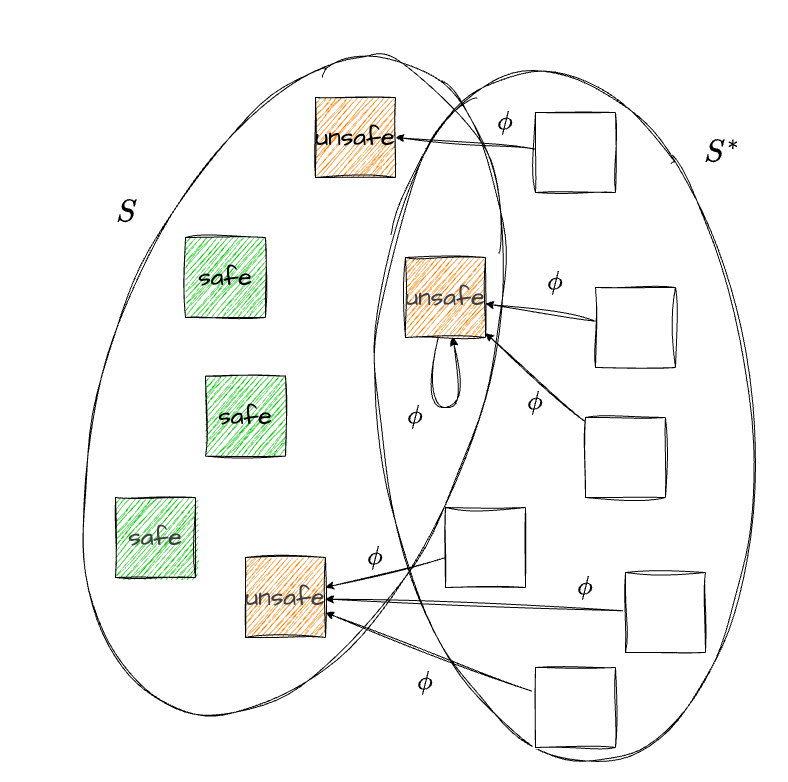
\includegraphics[width=\textwidth]{figures/safe-facility.drawio.png}
      \end{figure}
    \end{column}
    \begin{column}{0.45\textwidth}
      \begin{definition}[安全な施設]
        施設 \(i \in S\) が\info{安全}であるとは、
        最適解の全ての施設 \(i^* \in S^*\) について、
        \[
          \phi(i^*) \neq i
        \]
        が成立することである。
      \end{definition}
      逆に、ある施設 \(i^* \in S^*\) について、
      \[
        \phi(i^*) = i
      \]
      が成立する場合、施設 \(i\) を\alert{安全でない}とよぶ。
    \end{column}
  \end{columns}

  \note{
    \begin{itemize}
      \item 削除操作をスムーズに説明できなかった場合のために、もう一度説明する
    \end{itemize}
  }
\end{frame}

\begin{frame}{準備：安全でない施設 \(i\) に対する集合 \(R_i\) と施設 \(i'\)}
  \begin{columns}
    \begin{column}{0.45\textwidth}
      \begin{figure}
        \centering
        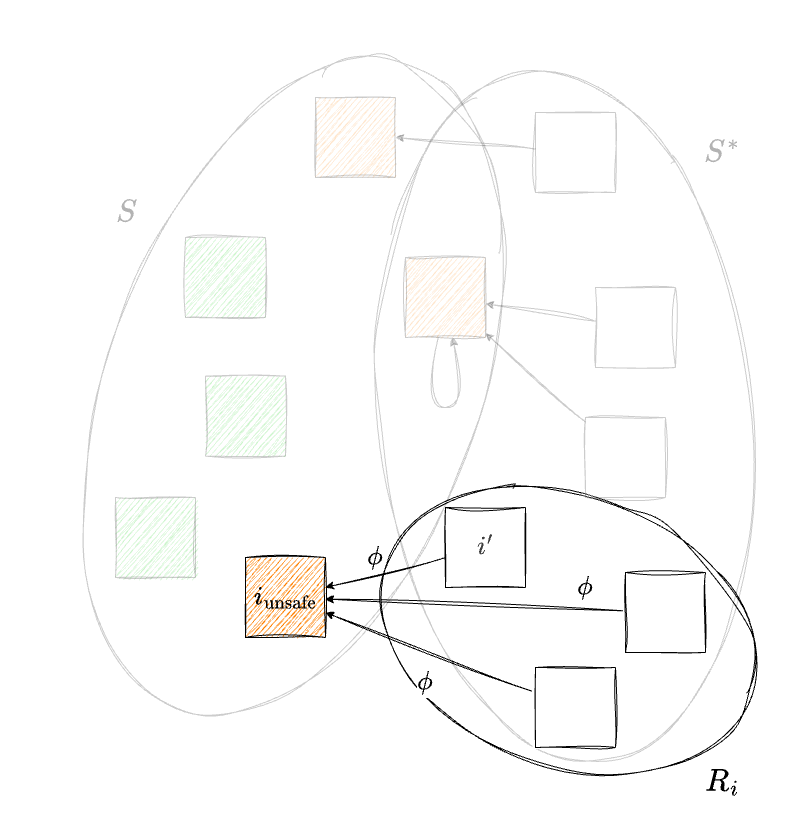
\includegraphics[width=\textwidth]{figures/Ri.drawio.png}
      \end{figure}
    \end{column}
    \begin{column}{0.45\textwidth}
      \begin{itemize}
        \item 安全でない施設 \(\alert{i_{\text{unsafe}}} \in S\) を固定する
        \item 最適解の施設 \(i^* \in S^*\) であって、\(\phi(i^*) = \alert{i_{\text{unsafe}}}\) を満たすものを \(R_{\alert{i_{\text{unsafe}}}} (\subseteq S^*)\) とする
              \begin{itemize}
                \item \(\alert{\alert{i_{\text{unsafe}}}}\) は安全でない \(\Leftrightarrow R_i \neq \emptyset\)
              \end{itemize}
        \item さらに、\(\alert{\alert{i_{\text{unsafe}}}}\) に最も近い \(R_{\alert{i_{\text{unsafe}}}}\) の施設を \(i^{'}\) とする
      \end{itemize}
    \end{column}
  \end{columns}

  \note{
    \begin{itemize}
      \item 図の場合 (\(i \notin S^*\)) は、\(R_i \subseteq S^* \setminus S\)
      \item ちなみに、\(i' \in S^* \setminus S\) か、さもなければ、\(i' = i\)
    \end{itemize}
  }
\end{frame}

\begin{frame}{追加移動：\(S^*\) の施設の開設と割り当ての変化}
  \begin{columns}
    \begin{column}{0.45\textwidth}
      \begin{figure}
        \centering
        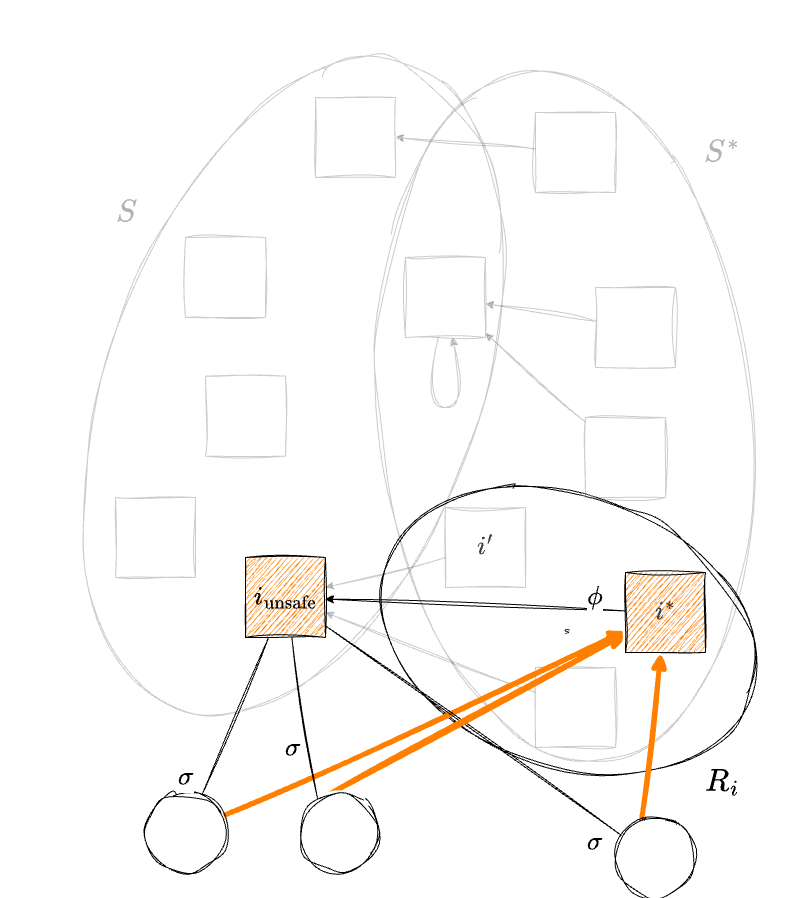
\includegraphics[width=\textwidth]{figures/unsafe-facility-add.drawio.png}
      \end{figure}
    \end{column}
    \begin{column}{0.45\textwidth}

      \only<1>{
        \begin{itemize}
          \item 施設 \(i^{*} \in {R_i \setminus \{i'\}}\) を開設する
          \item \(\localopt\) において \(\alert{i_{\text{unsafe}}}\) に割り当てられていた顧客のうち、\(\opt\) において \(i^{*}\) に割り当てられていた顧客を \(i^{*}\) に再割当てする
        \end{itemize}
      }
      \small{
        \only<2->{
          \vskip 0.5em
          次式が得られる：
          \begin{align*}
             & \underbrace{\sum_{i \in S} f_i + \sum_{j \in \DemandSet} c_{\sigma(j)j}}_{\text{局所最適解 } (S, \sigma) \text{ のコスト}}                                                                                                                                                                                 \\
             & \left(\le \underbrace{S \cup \{i^{*}\} \text{ の下で最適な割り当てをした解のコスト}}_{(S, \sigma) \text{ の近傍解のコスト}}\right)                                                                                                                                                                                          \\
             & \underbrace{\begin{aligned} \le \sum_{i \in S \cup \{i^{*}\}} f_i & +  \sum_{j \in \DemandSet \colon \sigma(j) \neq \alert{i_{\text{unsafe}}} \text{ or } \sigma^*(j) \neq i^{*}} c_{\sigma(j)j} \\
                                                      & + \sum_{j \in \DemandSet \colon \sigma(j) = \alert{i_{\text{unsafe}}} \text{ and } \sigma^*(j) = i^{*}} \alert{c_{i^{*}j}}
                             \end{aligned}}_{(S, \sigma) \text{ の近傍解の割り当てをいじった解のコスト}} \\
          \end{align*}
          \vskip -4.5em
        }
        \only<3>{
          \begin{align*}
            \Rightarrow 0 & \le f_{i^*} + \sum_{j \in \DemandSet \colon \sigma(j) = \alert{i_{\text{unsafe}}} \text{ and } \sigma^*(j) = i^{*}} (c_{i^{*}j} - c_{\sigma(j)j}) \\
          \end{align*}
        }
      }
    \end{column}
  \end{columns}
\end{frame}

\begin{frame}{【再掲】準備：安全でない施設 \(i\) に対する集合 \(R_i\) と施設 \(i'\)}
  \begin{columns}
    \begin{column}{0.45\textwidth}
      \begin{figure}
        \centering
        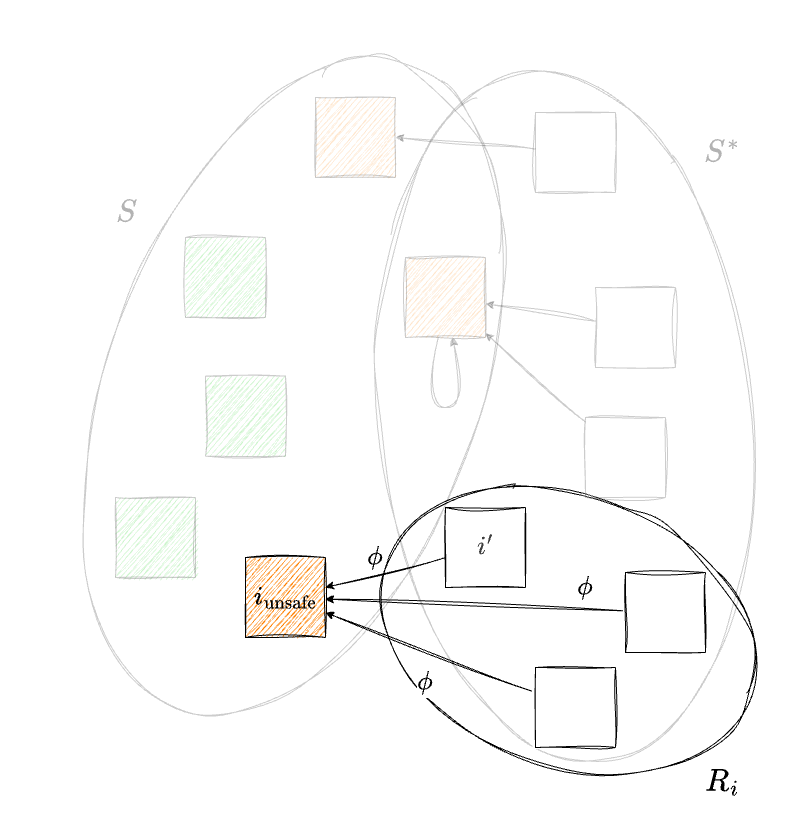
\includegraphics[width=\textwidth]{figures/Ri.drawio.png}
      \end{figure}
    \end{column}
    \begin{column}{0.45\textwidth}
      \begin{itemize}
        \item 安全でない施設 \(\alert{i_{\text{unsafe}}} \in S\) を固定する
        \item 最適解の施設 \(i^* \in S^*\) であって、\(\phi(i^*) = \alert{i_{\text{unsafe}}}\) を満たすものを \(R_{\alert{i_{\text{unsafe}}}} (\subseteq S^*)\) とする
              \begin{itemize}
                \item \(\alert{\alert{i_{\text{unsafe}}}}\) は安全でない \(\Leftrightarrow R_i \neq \emptyset\)
              \end{itemize}
        \item さらに、\(\alert{\alert{i_{\text{unsafe}}}}\) に最も近い \(R_{\alert{i_{\text{unsafe}}}}\) の施設を \(i^{'}\) とする
      \end{itemize}
    \end{column}
  \end{columns}

  \note{
    \begin{itemize}
      \item
    \end{itemize}
  }
\end{frame}

\begin{frame}{交換移動：\(S\) の安全でない施設と \(S^*\) の施設の交換と割り当ての変化}
  \begin{columns}
    \begin{column}{0.45\textwidth}
      \begin{figure}
        \centering
        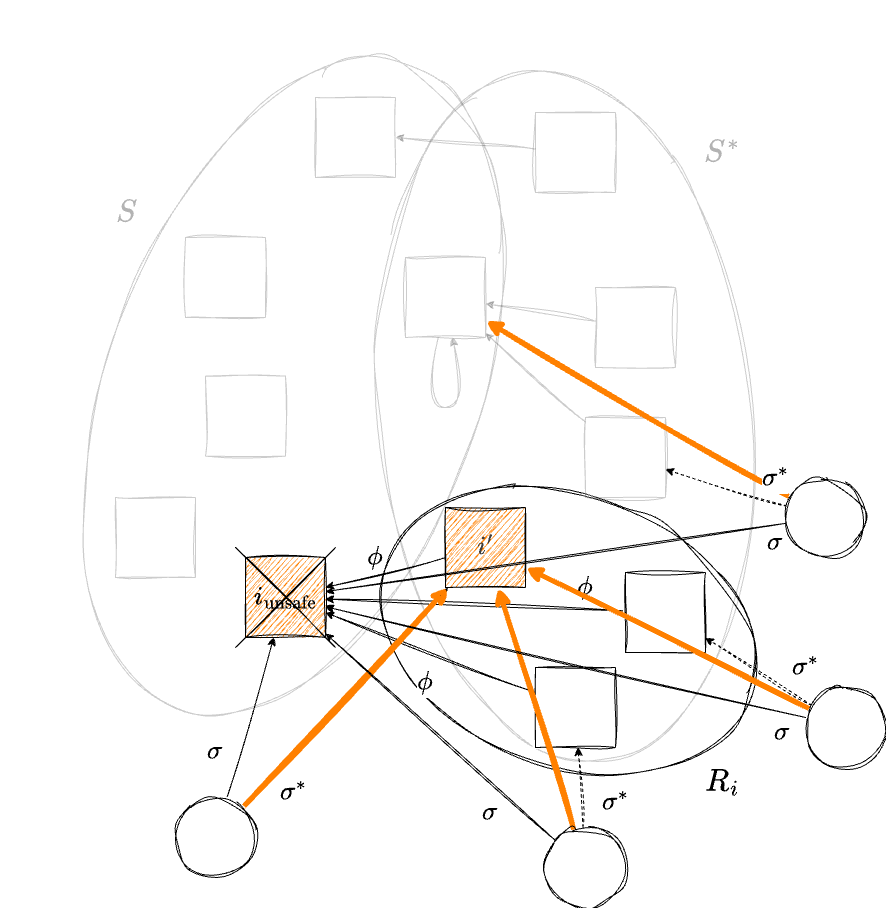
\includegraphics[width=\textwidth]{figures/unsafe-facility-swap.drawio.png}
      \end{figure}
    \end{column}
    \begin{column}{0.45\textwidth}
      \only<1>{
        \begin{itemize}
          \item \(\alert{i_{\text{unsafe}}}\) を閉鎖し、施設 \(i^{'}\) を開設
          \item \(\sigma(j) = i\) である利用者 \(j\) について割当てを変更：
                \begin{itemize}
                  \item \(\sigma^*(j) \in R_{\alert{i_{\text{unsafe}}}}\) であれば、\\\(j\) を \(i^{'}\) に再割当て
                  \item \(\sigma^*(j) \notin R_{\alert{i_{\text{unsafe}}}}\) であれば、\\\(j\) を \(\phi(\sigma^*(j))\) に再割当て
                \end{itemize}
        \end{itemize}
      }
      \small{
        \only<2>{
          % 次式が得られる：
          \begin{align*}
             & \underbrace{\sum_{i \in S} f_i + \sum_{j \in \DemandSet} c_{\sigma(j)j}}_{\text{局所最適解 } (S, \sigma) \text{ のコスト}}                                                                                           \\
             & \left(\le \underbrace{S \cup \{i^{'}\} \setminus \{\alert{i_{\text{unsafe}}}\} \text{ の下で最適な割り当てをした解のコスト}}_{(S, \sigma) \text{ の近傍解のコスト}}\right)                                                            \\
             & \underbrace{\begin{aligned}
                               \le \sum_{i \in S \cup \{i^{'}\} \setminus \{\alert{i_{\text{unsafe}}}\}} f_i
                                & + \sum_{j \in D \colon \sigma(j) \neq \alert{i_{\text{unsafe}}}} c_{\sigma(j)j}                                                                    \\
                                & + \sum_{j \in D \colon \sigma(j) = \alert{i_{\text{unsafe}}} \text{ and } \sigma^*(j) \in R_{\alert{i_{\text{unsafe}}}}} c_{i'j}                   \\
                                & + \sum_{j \in D \colon \sigma(j) = \alert{i_{\text{unsafe}}} \text{ and } \sigma^*(j) \notin R_{\alert{i_{\text{unsafe}}}}} c_{\phi(\sigma^*(j))j}
                             \end{aligned}}_{(S, \sigma) \text{ の近傍解の割り当てをいじった解のコスト}} \\
          \end{align*}
        }
        \only<3>{
          \begin{align*}
            \Rightarrow f_{\alert{i_{\text{unsafe}}}} & \le \begin{aligned}[t]
                                                              f_{i^{'}}
                                                               & + \sum_{j \in D \colon \sigma(j) = \alert{i_{\text{unsafe}}} \text{ and } \sigma^*(j) \in R_{\alert{i_{\text{unsafe}}}}} (c_{i'j} - c_{\sigma(j)j})                   \\
                                                               & + \sum_{j \in D \colon \sigma(j) = \alert{i_{\text{unsafe}}} \text{ and } \sigma^*(j) \notin R_{\alert{i_{\text{unsafe}}}}} (c_{\phi(\sigma^*(j))j} - c_{\sigma(j)j})
                                                            \end{aligned} \\
                                                      & \le \begin{aligned}[t]
                                                              f_{i^{'}}
                                                               & + \sum_{j \in D \colon \sigma(j) = \alert{i_{\text{unsafe}}} \text{ and } \sigma^*(j) \in R_{\alert{i_{\text{unsafe}}}}} (c_{i'j} - c_{\sigma(j)j})   \\
                                                               & + \sum_{j \in D \colon \sigma(j) = \alert{i_{\text{unsafe}}} \text{ and } \sigma^*(j) \notin R_{\alert{i_{\text{unsafe}}}}} \alert{2c_{\sigma^*(j)j}}
                                                            \end{aligned}
          \end{align*}
        }
      }
    \end{column}
  \end{columns}

  \note{
    \begin{itemize}
      \item 安全でない施設 \(\alert{i_{\text{unsafe}}}\) を \(S \bigcap S^*\) から選んだ場合、\(i' = \alert{i_{\text{unsafe}}}\) になる
    \end{itemize}
  }
\end{frame}

% \begin{frame}[standout]
%   \begin{figure}
%     \centering
%     
\includegraphics[width=0.3\textwidth]{figures/danger.png}
%   \end{figure}

%   次のスライドで大変ショッキングな数式が表示されます。

%   心臓の弱い方はご注意ください。
% \end{frame}

\begin{frame}{安全でない施設と \(S^*\) の施設に対する不等式}
  \only<1>{

    \begin{columns}
      \begin{column}{0.45\textwidth}
        \begin{figure}
          \centering
          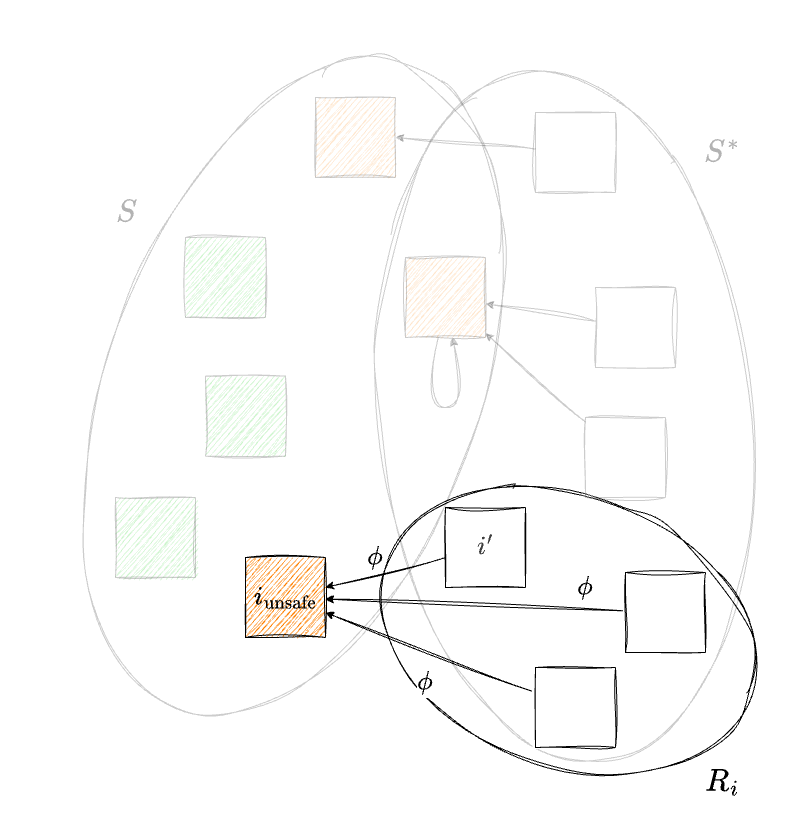
\includegraphics[width=\textwidth]{figures/Ri.drawio.png}
        \end{figure}
      \end{column}
      \begin{column}{0.45\textwidth}
        \vskip 1em

        \structure{追加移動 (\(i^* \in R_{\alert{i_{\text{unsafe}}}} \setminus \{i'\}\) に対して)}
        \begin{align*}
          0 & \le f_{i^*} + \sum_{j \in \DemandSet \colon \sigma(j) = \alert{i_{\text{unsafe}}} \text{ and } \sigma^*(j) = i^{*}} (c_{i^{*}j} - c_{\sigma(j)j}) \\
        \end{align*}

        \vskip -1em

        \structure{交換移動 (\(\alert{i_{\text{unsafe}}}\) ↔︎ \(i'\))}
        \begin{align*}
          f_{\alert{i_{\text{unsafe}}}} & \le \begin{aligned}[t]
                                                f_{i^{'}}
                                                 & + \sum_{j \in D \colon \sigma(j) = \alert{i_{\text{unsafe}}} \text{ and } \sigma^*(j) \in R_{\alert{i_{\text{unsafe}}}}} (c_{i'j} - c_{\sigma(j)j}) \\
                                                 & + \sum_{j \in D \colon \sigma(j) = \alert{i_{\text{unsafe}}} \text{ and } \sigma^*(j) \notin R_{\alert{i_{\text{unsafe}}}}} 2c_{\sigma^*(j)j}
                                              \end{aligned}
        \end{align*}

        \vskip -1em

        \[
          \Rightarrow f_{\iunsafe} \le \sum_{i^* \in R_{\iunsafe}} f_{i^*} + \sum_{j \in \DemandSet \colon \sigma(j) = \iunsafe} 2c_{\sigma^*(j)j}
        \]
      \end{column}
    \end{columns}
  }
  \only<2>{

    \(i^* \in R_i \setminus \{i^{'}\}\) に対する追加操作の不等式と交換操作の不等式を全て足し合わせると、
    \begin{align*}
      0 & \le \sum_{i^* \in R_i \setminus \{i'\}} \biggl( f_{i^*} + \sum_{j \in D \colon \sigma(j) = i \text{ and } \sigma^*(j) = i^*} (c_{\sigma^*(j)j} - c_{\sigma(j)j}) \biggr)                                                                                     \\
        & + \biggl( f_{i'} - f_i + \sum_{j \in D \colon \sigma(j) = i \text{ and } \sigma^*(j) \in R_i} (c_{i'j} - c_{\sigma(j)j}) + \sum_{j \in D \colon \sigma(j) = i \text{ and } \sigma^*(j) \notin R_i} 2c_{\sigma^*(j)j} \biggr)                                 \\
        & = - f_i + \sum_{i^* \in R_i} f_{i^*} + \sum_{j \in D \colon \sigma(j) = i \text{ and } \sigma^*(j) \notin R_i} 2c_{\sigma^*(j)j}                                                                                                                             \\
        & + \sum_{i^* \in R_i \setminus \{i'\}} \biggl(\sum_{j \in D \colon \sigma(j) = i \text{ and } \sigma^*(j) = i^*} (c_{\sigma^*(j)j} - c_{\sigma(j)j})\biggr) + \sum_{j \in D \colon \sigma(j) = i \text{ and } \sigma^*(j) \in R_i} (c_{i'j} - c_{\sigma(j)j}) \\
        & = - f_i + \sum_{i^* \in R_i} f_{i^*} + \sum_{j \in D \colon \sigma(j) = i \text{ and } \sigma^*(j) \notin R_i} 2c_{\sigma^*(j)j}                                                                                                                             \\
        & + \sum_{j \in D \colon \sigma(j) = i \text{ and } \sigma^*(j) \alert{\in R_i \setminus\{i^{'}\}}} (c_{\sigma^*(j)j} - c_{\sigma(j)j}) + \sum_{j \in D \colon \sigma(j) = i \text{ and } \sigma^*(j) \in R_i} (c_{i'j} - c_{\sigma(j)j})                      \\
    \end{align*}
  }
\end{frame}

\begin{frame}{がんばろう (2/2)}
  最後の二つの和に着目すると、
  \small{
    \begin{align*}
          & \sum_{j \in D \colon \sigma(j) = i \text{ and } \sigma^*(j) \in R_i \setminus\{i^{'}\}} (c_{\sigma^*(j)j} - c_{\sigma(j)j}) + \sum_{j \in D \colon \sigma(j) = i \text{ and } \sigma^*(j) \in R_i} (c_{i'j} - c_{\sigma(j)j})                                        \\
      =   & \sum_{j \in D \colon \sigma(j) = i \text{ and } \alert{\sigma^*(j) \in R_i \setminus\{i^{'}\}}} (c_{\sigma^*(j)j} + c_{i'j} - 2c_{\sigma(j)j}) + \sum_{j \in D \colon \sigma(j) = i \text{ and } \alert{\sigma^*(j) = i^{'}}} (c_{i'j} - c_{\sigma(j)j})             \\
      \le & \sum_{j \in D \colon \sigma(j) = i \text{ and } \sigma^*(j) \in R_i \setminus\{i^{'}\}} (c_{\sigma^*(j)j} + c_{i'j} - 2c_{\sigma(j)j}) + \sum_{j \in D \colon \sigma(j) = i \text{ and } \sigma^*(j) = i^{'}} \alert{2c_{\sigma^*(j)j}}                              \\
      \le & \sum_{j \in D \colon \sigma(j) = i \text{ and } \sigma^*(j) \in R_i \setminus\{i^{'}\}} (c_{\sigma^*(j)j} + \alert{(c_{\sigma^*(j)j} + 2c_{\sigma(j)j})} - 2c_{\sigma(j)j}) + \sum_{j \in D \colon \sigma(j) = i \text{ and } \sigma^*(j) = i^{'}} 2c_{\sigma^*(j)j} \\
      =   & \sum_{j \in D \colon \sigma(j) = i \text{ and } \sigma^*(j) \in R_i \setminus\{i^{'}\}} 2c_{\sigma^*(j)j} + \sum_{j \in D \colon \sigma(j) = i \text{ and } \sigma^*(j) = i^{'}} 2c_{\sigma^*(j)j}                                                                   \\
      =   & \sum_{j \in D \colon \sigma(j) = i \text{ and } \sigma^*(j) \in R_i} 2c_{\sigma^*(j)j}
    \end{align*}
  }
\end{frame}

\begin{frame}{そしてついに}
  よって、
  \[
    0 \le - f_i + \sum_{i^* \in R_i} f_{i^*} + \sum_{j \in D \colon \sigma(j) = i} 2c_{\sigma^*(j)j}
  \]
  が成立する。

  両辺を \(f_i\) で割り、全ての安全でない施設 \(i \in S\) について和を取ると、
  \[
    \sum_{i \in S \colon i \text{ is unsafe}} f_i \le \sum_{i \in S \colon i \text{ is unsafe}} \sum_{i^* \in R_i} f_{i^*} + \sum_{i \in S \colon i \text{ is unsafe}} \sum_{j \in D \colon \sigma(j) = i} 2c_{\sigma^*(j)j}
  \]

  最後に、左辺は \(F\) の安全でない施設部分を表し、右辺の第 1 項は \(F^*\) に対応し、第 2 項は \(2C^*\) に対応することに注意すると、補題が示されたことになる。
\end{frame}

\begin{frame}[standout]
  Break time!
\end{frame}

\section{改良された局所探索アルゴリズム}

\begin{frame}{施設配置問題に対する改良された局所探索アルゴリズム}
  \begin{theorem}[\cite{charikar2005improved}]
    施設配置問題に対して，任意の定数 \(\varepsilon > 0\) に対し，
    \alert{\(\tilde{\mathcal{O}}(n^2/\varepsilon)\)} 時間で \alert{\(1 + \sqrt{2} + \varepsilon\)} 倍の近似解を求めるスキームが存在する．
  \end{theorem}

  \textbf{Key idea. }
  \begin{itemize}
    \item 開設コストを適切にスケール
    \item 近傍への移動による改善が \(\varepsilon\) 未満であれば終了
  \end{itemize}
\end{frame}

\begin{frame}{改良点①：開設コストのスケーリング}
  \begin{itemize}
    \item 任意の定数 \(\mu > 0\) に対し、各施設 \(i\) の開設コストを
          \[
            f_i' = f_i / \mu
          \]
          でスケール
    \item 局所探索アルゴリズムをスケーリング後の開設コスト \(f_i'\) を用いて実行し、解 \((S, \sigma)\) を得る。
    \item 最終的な解のコストは、
          \[
            \sum_{i \in S} f_i + \sum_{j \in D} c_{\sigma(j)j} = (1 + \varepsilon) \sum_{i \in S} f_i' + \sum_{j \in D} c_{\sigma(j)j}
          \]
          である。
  \end{itemize}

\end{frame}

\section{まとめ}

\begin{frame}{施設配置問題に対する近似アルゴリズム}
  \begin{table}[]
    \centering
    \begin{tabular}{lcc}
      \toprule
      アルゴリズム                              & 近似比                     & 計算量                                      \\
      \midrule
      確定的ラウンディング                          & 4                       & ?                                        \\
      乱択ラウンディング                           & 3 (期待値)                 & ?                                        \\
      主双対法                                & 3                       &                                          \\
      貪欲法 (双対フィット法による解析)                  & 2                       &                                          \\
      貪欲法 (きわめて複雑な解析)                     & 1.61                    &                                          \\
      局所探索法~(\cite{arya2004local})        & 3                       &                                          \\
      局所探索法~(\cite{charikar2005improved}) & \(2.414 + \varepsilon\) & \(\tilde{\mathcal{O}}(n^2/\varepsilon)\) \\
      \cite{li2013a}                      & 1.488                   &                                          \\
      \bottomrule
    \end{tabular}
  \end{table}

  また \(\mathcal{P} \neq \mathcal{NP}\) のもとで、1.463-近似アルゴリズムが存在しないことが知られている。
\end{frame}

\begin{frame}[allowframebreaks]{References}
  \printbibliography[heading=none]{}
\end{frame}

\end{document}
